% =============================================================================
%  IEEE conference paper: LLM farm-manager agent on a plant-growth digital twin
%
%  IMPORTANT, READ BEFORE SUBMITTING
%  Every value wrapped in \ph{...} (shown in RED in the PDF) is a PLACEHOLDER for
%  the LLM agent, which has not been evaluated yet. Agent series in the figures
%  are drawn DASHED / HATCHED and marked with a dagger for the same reason.
%  All other numbers are real: the ML metrics come from generate_and_train_v2.py
%  and the no-intervention / rule-based results from 50 runs of evaluate.py.
%
%  To finish the paper:
%    1. python evaluate.py --seeds 5 --include-agent
%    2. Copy the "LLM agent" values from runs/eval/METRICS.md into every \ph{...}
%       and into the coordinates marked % PLACEHOLDER in the figures.
%    3. Remove the red notice box below and change \ph to: \newcommand{\ph}[1]{#1}
%    4. Rewrite any sentence in the Results/Discussion that the real numbers contradict.
% =============================================================================
\documentclass[conference]{IEEEtran}
\IEEEoverridecommandlockouts

\usepackage{cite}
\usepackage{amsmath,amssymb,amsfonts}
\usepackage{graphicx}
\usepackage{textcomp}
\usepackage{xcolor}
\usepackage{booktabs}
\usepackage{multirow}
\usepackage{array}
\usepackage{tikz}
\usetikzlibrary{arrows.meta,positioning,fit,backgrounds,patterns}
\usepackage{pgfplots}
\usepgfplotslibrary{groupplots}
\pgfplotsset{compat=1.17}
\usepackage[hidelinks]{hyperref}

% ----- colours (fixed per policy across every figure) -----
\definecolor{cNone}{HTML}{2A78D6}
\definecolor{cRule}{HTML}{EB6834}
\definecolor{cAgent}{HTML}{1BAF7A}
\definecolor{cEvent}{HTML}{EDA100}
\definecolor{cInk}{HTML}{3D3D3A}

% ----- placeholder marker: red now, make it a no-op once real values are in -----
\newcommand{\ph}[1]{\textcolor{red}{#1}}
\newcommand{\agentmark}{$^{\dagger}$}

\pgfplotsset{
  every axis/.append style={
    font=\scriptsize, axis line style={cInk!60}, tick style={cInk!60},
    label style={font=\scriptsize}, tick label style={font=\scriptsize},
    legend style={font=\scriptsize, draw=none, fill=none},
    ymajorgrids, grid style={cInk!12},
  },
}

\begin{document}

\title{An Autonomous LLM Agent for Crop Management in a\\Plant-Growth Digital Twin Under Weather Disturbances}

\author{\IEEEauthorblockN{Rishabh Arya}
\IEEEauthorblockA{\textit{Department of Computer Science and Engineering (AI \& ML)}\\
\textit{Dayananda Sagar University}\\
Bengaluru, India\\
rishabharya.k@gmail.com}
% \and
% \IEEEauthorblockN{Second Author}
% \IEEEauthorblockA{\textit{Department of Computer Science and Engineering (AI \& ML)}\\
% \textit{Dayananda Sagar University}\\
% Bengaluru, India\\
% email@example.com}
}

\maketitle

% ---------------------------------------------------------------- draft notice
\noindent\fcolorbox{red}{red!5}{\parbox{0.95\columnwidth}{\footnotesize\color{red}
\textbf{DRAFT.} Values in red and figure series marked \agentmark{} are placeholders
for the LLM agent pending experiments. Replace before submission.}}
\vspace{2pt}

\begin{abstract}
Digital twins promise data-driven crop management, but full agricultural twins require dense
sensor networks that are impractical for small farms and for research prototyping. We present a
parameter-driven plant-growth digital twin built in Unity3D and an autonomous large language model
(LLM) agent that manages it. The twin maps six environmental variables (soil pH, soil moisture,
sunlight, temperature, humidity and rainfall) to a daily growth score, which drives a 144-plant,
seven-stage 3D crop simulation. A gradient-boosting surrogate of the growth response, trained on
18{,}000 balanced synthetic samples with isotonic calibration, reaches $R^2 = 0.984$ and
RMSE $= 0.053$. The agent interacts with the twin over a local HTTP interface through four tools
(observe, simulate a what-if change, actuate, and advance time) under actuator limits, with
temperature and rainfall left uncontrollable. Crucially, it is not given the crop's optimal ranges
and must discover them by querying the twin. Across five weather scenarios and five seeds, an
unmanaged farm dies in 60\% of seasons. A rule-based controller with privileged knowledge of the
optimal ranges reaches 100\% success. The LLM agent reaches \ph{96\%} success without that knowledge,
reacting to weather events in \ph{1.0} day on average versus 3.1 days for the rule-based controller,
at a cost of \ph{41} model calls per season.
\end{abstract}

\begin{IEEEkeywords}
digital twin, LLM agents, tool use, precision agriculture, gradient boosting, simulation, Unity
\end{IEEEkeywords}

% =============================================================================
\section{Introduction}
% =============================================================================

A digital twin is a virtual representation of a physical system that mirrors its state and
behaviour and can be used to test interventions before applying them to the real
system~\cite{grieves2017digital}. In agriculture, twins have been proposed for irrigation
scheduling, yield forecasting and farm-level decision support~\cite{verdouw2021digital,
pylianidis2021introducing}. Two obstacles limit their practical use. First, a faithful twin needs
continuous sensing of soil, plant and weather state, which is costly to deploy. Second, a twin only
produces value when someone reads it and acts on it; most farm decision-support systems still
leave diagnosis and planning to a human expert.

Mechanistic crop models such as DSSAT~\cite{jones2003dssat} and AquaCrop~\cite{steduto2009aquacrop}
address the first obstacle by simulating crop response from environmental inputs. Machine learning
has been applied widely to yield and stress prediction~\cite{liakos2018machine,
kamilaris2018deep}, and reinforcement learning has been studied for crop management
policies~\cite{gautron2022reinforcement}, although RL policies require many simulated seasons to
train and transfer poorly when the environment changes. Meanwhile, LLM-based agents that reason in
natural language and act through tools have shown strong zero-shot performance on open-ended
tasks~\cite{yao2023react,schick2023toolformer,wang2024survey}. This raises a question we
investigate here: \emph{can a general-purpose LLM agent, given only tool access to a digital twin
and no task-specific training, keep a crop alive and productive under unannounced weather
disturbances?}

We make four contributions:
\begin{enumerate}
  \item A parameter-driven plant-growth digital twin in Unity3D with a 144-plant, seven-stage
        visual crop, day--night lighting and an interactive control panel, exposed to external
        agents through a local HTTP API (Section~\ref{sec:twin}).
  \item A calibrated gradient-boosting surrogate of the crop's growth response, trained on a
        balanced synthetic dataset and exportable to ONNX for in-engine inference
        (Section~\ref{sec:model}).
  \item A tool-using LLM farm-manager agent that observes, diagnoses with what-if queries on the
        twin, actuates under equipment limits and paces its own control loop
        (Section~\ref{sec:agent}).
  \item An evaluation harness with five weather scenarios, two baselines and metrics for outcome,
        crop health, resilience, efficiency and agent behaviour (Sections~\ref{sec:setup}
        and~\ref{sec:results}).
\end{enumerate}

% =============================================================================
\section{Related Work}
% =============================================================================

\textbf{Digital twins in agriculture.} Verdouw \emph{et al.}~\cite{verdouw2021digital} define a
reference architecture for smart-farming twins and note that most reported systems are at the
monitoring stage, with few closing the loop to automated control. Pylianidis
\emph{et al.}~\cite{pylianidis2021introducing} review agricultural twins and identify the cost of
sensing and the lack of decision layers as key gaps. Our twin is deliberately sensor-free: state
is supplied by a user or an agent, which makes it suitable for prototyping control strategies.

\textbf{Crop models and ML.} Process-based models~\cite{jones2003dssat,steduto2009aquacrop}
encode crop physiology in detail but require extensive calibration. Data-driven methods trade
physiological fidelity for flexibility~\cite{liakos2018machine,kamilaris2018deep}. For tabular
inputs such as ours, tree ensembles remain competitive with deep networks~\cite{grinsztajn2022tree};
we use gradient boosting~\cite{friedman2001greedy} with isotonic
calibration~\cite{zadrozny2002transforming}.

\textbf{Learning-based crop control.} RL has been applied to fertilisation and irrigation
decisions in crop simulators~\cite{gautron2022reinforcement}. RL agents learn effective policies
but need many training episodes~\cite{sutton2018reinforcement} and offer no natural-language
rationale for their actions.

\textbf{LLM agents.} ReAct~\cite{yao2023react} interleaves reasoning traces with tool actions;
Toolformer~\cite{schick2023toolformer} shows that language models can learn when to call APIs;
Reflexion~\cite{shinn2023reflexion} adds verbal self-reflection across episodes; and
Voyager~\cite{wang2023voyager} demonstrates open-ended embodied control in a game environment. Unity
has previously served as a platform for learning agents through ML-Agents~\cite{juliani2018unity}.
To our knowledge, this work is among the first to evaluate a tool-using LLM agent as a closed-loop
controller on an agricultural digital twin against both an unmanaged and a privileged rule-based
baseline.

% =============================================================================
\section{System Architecture}
% =============================================================================

Fig.~\ref{fig:arch} shows the system. The Unity application hosts the twin and an HTTP server.
A Python environment layer sits between the agent and the twin, enforcing the rules of the
task (which variables are controllable, by how much per action) and injecting weather events.
The same Python layer can drive a headless replica of the growth logic, which reproduces the
Unity simulation exactly and is used for batch evaluation.

\begin{figure*}[t]
\centering
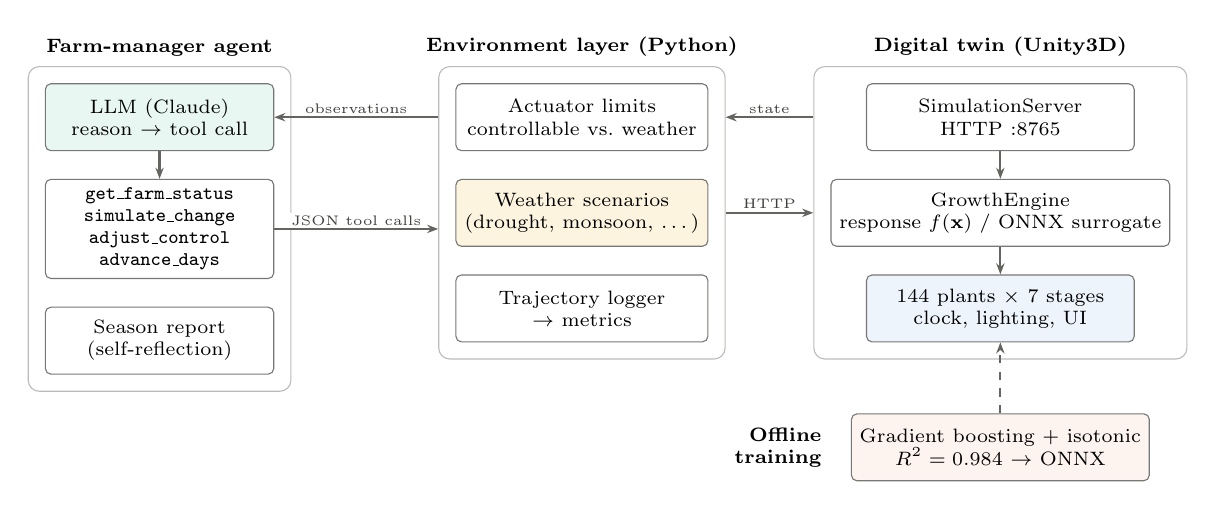
\begin{tikzpicture}[
  font=\scriptsize,
  box/.style={draw=cInk!70, rounded corners=2pt, fill=white, align=center,
              minimum height=0.85cm, inner sep=3pt},
  grp/.style={draw=cInk!35, rounded corners=4pt, inner sep=6pt},
  arr/.style={-{Stealth[length=4pt]}, cInk!80, thick},
  lbl/.style={font=\tiny, text=cInk, align=center, fill=white, inner sep=1pt}]

  % --- agent column
  \node[box, fill=cAgent!10, minimum width=2.9cm] (llm) {LLM (Claude)\\reason $\rightarrow$ tool call};
  \node[box, below=0.35cm of llm, minimum width=2.9cm] (tools)
       {\texttt{get\_farm\_status}\\\texttt{simulate\_change}\\\texttt{adjust\_control}\\\texttt{advance\_days}};
  \node[box, below=0.35cm of tools, minimum width=2.9cm] (report) {Season report\\(self-reflection)};
  \begin{scope}[on background layer]
    \node[grp, fit=(llm)(tools)(report), label={[font=\scriptsize\bfseries]above:Farm-manager agent}] (gA) {};
  \end{scope}

  % --- environment column
  \node[box, right=2.3cm of llm, minimum width=3.2cm] (rules) {Actuator limits\\controllable vs.\ weather};
  \node[box, below=0.35cm of rules, minimum width=3.2cm, fill=cEvent!12] (weather) {Weather scenarios\\(drought, monsoon, \dots)};
  \node[box, below=0.35cm of weather, minimum width=3.2cm] (log) {Trajectory logger\\$\rightarrow$ metrics};
  \begin{scope}[on background layer]
    \node[grp, fit=(rules)(weather)(log), label={[font=\scriptsize\bfseries]above:Environment layer (Python)}] (gE) {};
  \end{scope}

  % --- unity column
  \node[box, right=2.0cm of rules, minimum width=3.4cm] (server) {SimulationServer\\HTTP :8765};
  \node[box, below=0.35cm of server, minimum width=3.4cm] (engine) {GrowthEngine\\response $f(\mathbf{x})$ / ONNX surrogate};
  \node[box, below=0.35cm of engine, minimum width=3.4cm, fill=cNone!8] (scene) {144 plants $\times$ 7 stages\\clock, lighting, UI};
  \begin{scope}[on background layer]
    \node[grp, fit=(server)(engine)(scene), label={[font=\scriptsize\bfseries]above:Digital twin (Unity3D)}] (gU) {};
  \end{scope}

  % --- offline ML
  \node[box, below=0.9cm of scene, minimum width=3.4cm, fill=cRule!8] (ml) {Gradient boosting + isotonic\\$R^2=0.984$ $\rightarrow$ ONNX};
  \node[left=0.25cm of ml, font=\scriptsize\bfseries, align=right] {Offline\\training};

  % --- arrows
  \draw[arr] (llm) -- (tools);
  \draw[arr] (tools.east) -- node[lbl, above]{JSON tool calls} (gE.west |- tools.east);
  \draw[arr] (gE.east |- weather.east) -- node[lbl, above]{HTTP} (gU.west |- engine.west);
  \draw[arr] (gU.west |- server.west) -- node[lbl, above]{state} (gE.east |- rules.east);
  \draw[arr] (gE.west |- rules.west) -- node[lbl, above]{observations} (llm.east);
  \draw[arr] (server) -- (engine);
  \draw[arr] (engine) -- (scene);
  \draw[arr, dashed] (ml) -- (scene.south);
\end{tikzpicture}
\caption{System overview. The agent acts only through tools mediated by the environment layer,
which enforces actuator limits and applies weather events. The twin answers state, what-if and
time-advance requests over HTTP; the trained surrogate is exported to ONNX for in-engine use.}
\label{fig:arch}
\end{figure*}

% =============================================================================
\section{Plant-Growth Digital Twin}\label{sec:twin}
% =============================================================================

\subsection{Environmental State}
The environment is a vector $\mathbf{x} = (x_{\text{pH}}, x_{\text{SM}}, x_{\text{sun}},
x_{T}, x_{\text{RH}}, x_{\text{rain}})$ of soil pH, soil moisture (\%), sunlight (h/day),
temperature (\textdegree C), relative humidity (\%) and rainfall (mm/day).
Table~\ref{tab:features} lists the ranges, which are modelled on a tomato-like crop.

\begin{table}[t]
\centering
\caption{Environmental Variables and Response Parameters}
\label{tab:features}
\footnotesize
\setlength{\tabcolsep}{3pt}
\begin{tabular}{@{}lcccc@{}}
\toprule
Variable & Hard range & Optimal & $w_j$ & Control/action \\
\midrule
pH                  & 3.5--9.5  & 6.0--7.0 & 1.0 & $\pm$0.5 \\
Soil moisture (\%)  & 5--100    & 40--70   & 1.4 & $\pm$20 \\
Sunlight (h/day)    & 0--16     & 6--10    & 1.2 & $\pm$3 \\
Temperature (\textdegree C) & 0--45 & 20--30 & 1.4 & weather \\
Humidity (\%)       & 10--100   & 50--75   & 0.9 & $\pm$15 \\
Rainfall (mm/day)   & 0--120    & 20--60   & 1.1 & weather \\
\bottomrule
\end{tabular}
\end{table}

\subsection{Growth Response Function}
Each variable is scored by a piecewise bell function with optimal band $[a_j, b_j]$ and hard
limits $[l_j, u_j]$:
\begin{equation}
\phi_j(x) =
\begin{cases}
0 & x \le l_j \ \text{or}\ x \ge u_j \\[2pt]
0.85 + 0.15\left(1 - \dfrac{|x - m_j|}{h_j}\right) & a_j \le x \le b_j \\[6pt]
1 - \left(\dfrac{a_j - x}{a_j - l_j}\right)^{1.8} & l_j < x < a_j \\[6pt]
1 - \left(\dfrac{x - b_j}{u_j - b_j}\right)^{1.8} & b_j < x < u_j
\end{cases}
\end{equation}
where $m_j$ and $h_j$ are the midpoint and half-width of the optimal band. Scores are combined
by a weighted mean, and a critical-failure penalty ensures that a single limiting factor
(for example, zero sunlight) cannot be averaged away:
\begin{equation}
r = \frac{1}{7}\sum_j w_j\,\phi_j, \qquad
s = \begin{cases}
0.5\, r \left(\phi_{\min}/0.2\right)^{1.5} & \phi_{\min} < 0.2 \\
r & \text{otherwise}
\end{cases}
\end{equation}
The daily growth score $s \in [0,1]$ is interpreted as deteriorating ($s<0.5$) or growing
($s \ge 0.5$).

\subsection{Crop Dynamics}
Each plant $i$ holds a progress value $p_i \in [0,1]$ and a fixed offset
$\varepsilon_i \sim \mathcal{U}(-0.05, 0.05)$ that models natural variation across the field.
Each simulated day,
\begin{equation}
p_i \leftarrow \operatorname{clip}_{[0,1]}\!\left(p_i + \Delta(\tilde s_i)\right),\quad
\tilde s_i = \operatorname{clip}_{[0,1]}(s + \varepsilon_i),
\end{equation}
\begin{equation}
\Delta(\tilde s) =
\begin{cases}
0.04\,(\tilde s - 0.5) & \tilde s \ge 0.5\\
-0.03\,(0.5 - \tilde s) & \tilde s < 0.5.
\end{cases}
\end{equation}
Under ideal conditions a plant therefore gains at most 2\% progress per day. Growth stage is
$k_i = \lfloor 7 p_i \rfloor$. The crop has \emph{matured} when the field mean $\bar p \ge 0.98$
and has \emph{died} when $\bar p$ returns to zero after having exceeded 0.05. The twin also
reports a forecast of days to maturity, $(0.98 - \bar p)/\Delta(s)$, or to death,
$\bar p/|\Delta(s)|$, under current conditions.

\subsection{Unity Implementation}
The scene contains a 12$\times$12 grid of plants spaced 1.5\,m apart. Each plant is a prefab
with seven stage meshes from a photogrammetry asset. Within a stage the active mesh scales
smoothly with progress; at a stage boundary the next mesh scales in from zero before the previous
one is disabled, which avoids visible popping. Plant colour is set per instance through material
property blocks, moving from deep green ($s > 0.65$) through yellow to brown ($s < 0.35$). A
simulation clock emits a day event consumed by the growth engine, the day--night lighting cycle
and the UI. On an Apple M1 laptop a 12$\times$12 grid ran smoothly, whereas a 50$\times$50 grid
(2{,}500 plants) produced frame times of about 1.5\,s once most plants reached the later,
higher-polygon growth stages, so 144 plants were used throughout.

\textbf{Agent interface.} A \texttt{SimulationServer} component exposes \texttt{GET /state},
\texttt{POST /environment}, \texttt{POST /predict} (what-if, no side effects),
\texttt{POST /advance}, \texttt{POST /reset} and \texttt{POST /log}. Requests arrive on a
background thread and are executed on Unity's main thread through a queue. While the agent
controls time, the real-time clock is paused and days are stepped explicitly, with a short
delay so that growth remains visible. Agent changes are routed through the UI sliders, so an
observer sees the controls move, and the agent's reasoning is shown in an on-screen log.

% =============================================================================
\section{Learned Growth Surrogate}\label{sec:model}
% =============================================================================

\subsection{Dataset}
No public dataset covers all six variables at daily resolution with a health label, so we
generated 18{,}000 labelled samples from an extended response function that additionally includes
growth-stage sensitivity (seedlings are penalised more heavily) and a compounding penalty when two
or more variables are stressed. To avoid the label imbalance observed in an initial uniform sample,
the data were drawn in three equal strata: stressed conditions, near-optimal conditions and
uniform sampling over the full ranges. Gaussian label noise ($\sigma = 0.012$) was added to
discourage memorisation of the formula. The final set contains 9{,}432 deteriorating and
8{,}568 growing samples, split 72/13/15 into training, calibration and test sets.

\subsection{Model and Calibration}
An initial random forest exhibited regression toward the mean, predicting approximately 0.6 for
most true scores between 0.3 and 0.8. We therefore used gradient
boosting~\cite{friedman2001greedy} (300 trees, depth 5, learning rate 0.04, subsample 0.8)
followed by isotonic regression~\cite{zadrozny2002transforming} fitted on the calibration split,
which stretches predictions back toward the extremes.

\begin{table}[t]
\centering
\caption{Surrogate Model Performance on the Held-Out Test Set ($n=2{,}700$)}
\label{tab:ml}
\footnotesize
\begin{tabular}{@{}lcc@{}}
\toprule
Metric & Gradient boosting & GB + isotonic \\
\midrule
$R^2$                   & 0.967 & \textbf{0.984} \\
RMSE                    & 0.076 & \textbf{0.053} \\
Std.\ of predictions    & 0.405 & 0.415 \\
Std.\ of targets        & \multicolumn{2}{c}{0.417} \\
\bottomrule
\end{tabular}
\end{table}

Table~\ref{tab:ml} shows that calibration reduces RMSE by 31\% and brings the spread of
predictions close to that of the targets. Fig.~\ref{fig:mleval} shows predicted-versus-actual
scores and the score distributions; Table~\ref{tab:sanity} lists predictions for hand-crafted
scenarios.

\begin{figure*}[t]
\centering
\includegraphics[width=0.92\textwidth]{model_evaluation.png}
\caption{Surrogate evaluation. Top: predicted versus actual growth score before and after
isotonic calibration, and impurity-based feature importance. Bottom: score distributions,
residuals, and predicted score by growth stage.}
\label{fig:mleval}
\end{figure*}

\begin{table}[t]
\centering
\caption{Calibrated Predictions for Hand-Crafted Conditions}
\label{tab:sanity}
\footnotesize
\setlength{\tabcolsep}{4pt}
\begin{tabular}{@{}lcl@{}}
\toprule
Condition & Score & Zone \\
\midrule
All variables optimal          & 0.923 & growing \\
Optimal, seed stage            & 0.895 & growing \\
Drought (SM 10\%, rain 2\,mm)  & 0.120 & deteriorating \\
Waterlogged (SM 95\%, rain 110\,mm) & 0.312 & deteriorating \\
No sunlight                    & 0.177 & deteriorating \\
Multiple stresses              & 0.006 & deteriorating \\
Heat stress (42\,\textdegree C)& 0.714 & growing (slow) \\
Acidic soil (pH 4.0)           & 0.758 & growing (slow) \\
\bottomrule
\end{tabular}
\end{table}

\textbf{Feature importance.} Fig.~\ref{fig:fi} reports impurity-based importances. Sunlight and
humidity dominate, even though the response function weights soil moisture and temperature most
heavily. This is an artefact of the stratified sampling: in the stressed stratum, sunlight
(0--3\,h) and humidity (10--28\%) are \emph{always} drawn from their stress ranges, whereas the
other variables are drawn from one of two tails. Those two features therefore separate the
strata almost perfectly. We report this because importance from a synthetic dataset reflects
the sampling design as much as the underlying physiology, and should not be read as an
agronomic finding.

\begin{figure}[t]
\centering
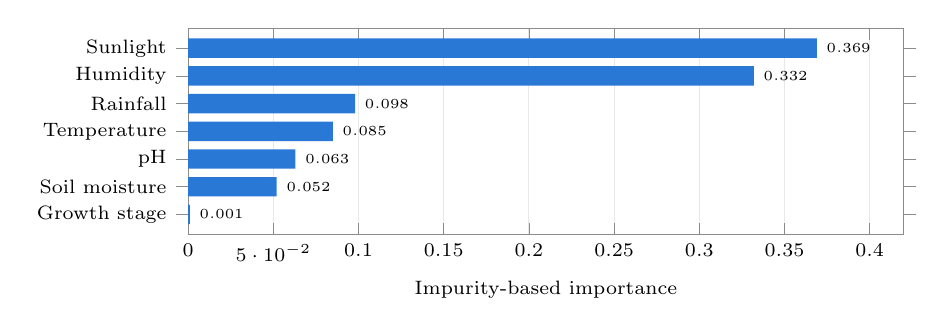
\begin{tikzpicture}
\begin{axis}[
  xbar, width=0.88\columnwidth, height=4.2cm,
  bar width=7pt, xmin=0, xmax=0.42, enlarge y limits=0.12,
  xlabel={Impurity-based importance},
  symbolic y coords={Growth stage,Soil moisture,pH,Temperature,Rainfall,Humidity,Sunlight},
  ytick=data, xmajorgrids, ymajorgrids=false,
  nodes near coords, nodes near coords style={font=\tiny, /pgf/number format/fixed,
    /pgf/number format/precision=3},
]
\addplot[fill=cNone, draw=none] coordinates {
  (0.001,Growth stage) (0.052,Soil moisture) (0.063,pH) (0.085,Temperature)
  (0.098,Rainfall) (0.332,Humidity) (0.369,Sunlight)};
\end{axis}
\end{tikzpicture}
\caption{Feature importance of the gradient-boosting surrogate. The dominance of sunlight and
humidity is explained by the stratified sampling (see text).}
\label{fig:fi}
\end{figure}

% =============================================================================
\section{LLM Farm-Manager Agent}\label{sec:agent}
% =============================================================================

\subsection{Task}
The agent manages one season of up to 120 days. Its objectives, in priority order, are to keep
the crop alive, bring it to maturity as quickly as possible, and use as few equipment actions as
reasonably possible. It may control soil moisture (irrigation or drainage), pH (lime or sulfur),
sunlight (grow lights or shade netting) and humidity (misting or ventilation), each with a
maximum change per action (Table~\ref{tab:features}). Temperature and rainfall are weather: the
agent cannot change them and must compensate with the controls it has.

\subsection{Tools}
Table~\ref{tab:tools} lists the four tools. The design separates \emph{thinking} from
\emph{acting}: \texttt{simulate\_change} queries the twin for the score under hypothetical
conditions at no cost, while \texttt{adjust\_control} changes the field and is penalised by the
efficiency objective. \texttt{advance\_days} lets the agent choose its own control interval.

\begin{table}[t]
\centering
\caption{Agent Tools}
\label{tab:tools}
\footnotesize
\setlength{\tabcolsep}{4pt}
\begin{tabular}{@{}l>{\raggedright\arraybackslash}p{0.6\columnwidth}@{}}
\toprule
Tool & Behaviour \\
\midrule
\texttt{get\_farm\_status} & Day, score, health zone, growth rate, progress, stage, forecast outcome and days, environment, active weather. \\
\texttt{simulate\_change}  & Score and growth rate under hypothetical values for any variables. No side effects. \\
\texttt{adjust\_control}   & Moves one controllable variable toward a target, clipped to the actuator limit. Requires a stated reason. \\
\texttt{advance\_days}     & Advances 1--10 days, applying weather each day; returns weather news, score range and new status. \\
\bottomrule
\end{tabular}
\end{table}

\subsection{Information Asymmetry}
The agent's system prompt describes the objectives, the controls and their limits, and the
meaning of the growth score, but \emph{not} the optimal ranges in Table~\ref{tab:features}. The
agent must combine prior agronomic knowledge with what-if queries to locate them, for example by
evaluating the score with soil moisture at several values and choosing the best. This makes the
task a test of diagnosis and planning rather than of following a known rule.

\subsection{Control Loop}
The agent runs a ReAct-style loop~\cite{yao2023react}: observe, identify the limiting factor,
test candidate fixes with \texttt{simulate\_change}, act, then advance time. The prompt suggests
large steps (5--10 days) when conditions are stable and small steps (1--3 days) during weather
events or when $s < 0.6$, leaving the final choice to the agent. Each assistant turn may contain
several tool calls; results are returned in the next turn. At the end of the season the agent
writes a short report on what happened and what it would change, in the spirit of
Reflexion~\cite{shinn2023reflexion}. We used Claude Sonnet as the underlying model with a cap
of 150 model calls per season.

% =============================================================================
\section{Experimental Setup}\label{sec:setup}
% =============================================================================

\subsection{Scenarios}
Table~\ref{tab:scenarios} lists the five scenarios. Events set some variables on their first day,
apply a daily drift while active (for example, soil drying by 4 percentage points per day in a
drought), and restore normal weather on the following day. Seed 0 is the canonical scenario;
seeds 1--4 shift event timing by up to $\pm$3 days and scale drift by 0.85--1.15, so results
measure robustness rather than performance on one fixed script. Each policy was run on every
scenario with five seeds (25 seasons per policy).

\begin{table}[t]
\centering
\caption{Weather Scenarios (Canonical Timing)}
\label{tab:scenarios}
\footnotesize
\setlength{\tabcolsep}{4pt}
\begin{tabular}{@{}l>{\raggedright\arraybackslash}p{0.68\columnwidth}@{}}
\toprule
Scenario & Events \\
\midrule
Calm            & None (control case). \\
Drought         & Days 15--38: rain 3\,mm, 36\,\textdegree C; soil $-$4\%/day, humidity $-$2\%/day. \\
Monsoon         & Days 20--42: rain 110\,mm, humidity 92\%, sunlight 4\,h; soil $+$5\%/day. \\
Acid soil       & Starts at pH 4.4, soil 22\%, sunlight 4.5\,h; acid rain on day 30 (pH $-$1.2). \\
Heatwave\,+\,storm & Days 18--30: 41\,\textdegree C, rain 8\,mm, soil $-$3\%/day; days 40--47: rain 105\,mm, sunlight 3\,h, soil $+$6\%/day. \\
\bottomrule
\end{tabular}
\end{table}

\subsection{Baselines}
\textbf{No intervention} never acts and measures what the weather alone does to the crop.
\textbf{Rule-based} is a threshold controller that checks every three days and moves any
controllable variable outside its optimal band to the band's midpoint. It has privileged access
to the true optimal ranges, which the agent does not, so it is a strong baseline.

\subsection{Metrics}
\emph{Outcome}: success rate (matured within the season), death rate and days to maturity
(successful seasons only). \emph{Crop health}: mean daily score and \emph{stress days}
($s<0.5$). \emph{Efficiency}: equipment actions per season. \emph{Resilience}, per weather event:
\emph{score drop} (mean score in the three days before the event minus the minimum score in the
event window), \emph{progress lost}, and \emph{reaction time} (days from event start to the first
action). \emph{Agent behaviour}: model calls, tool calls, tool error rate and what-if queries per
action. Values are reported as mean~$\pm$~standard deviation over seeds.

% =============================================================================
\section{Results}\label{sec:results}
% =============================================================================

\subsection{Overall Performance}
Table~\ref{tab:overall} summarises all 75 seasons. Without management the crop dies in 60\% of
seasons: in every drought, monsoon and acid-soil run. The rule-based controller saves every season
and reduces mean stress days from 20.6 to 0.1. The LLM agent achieves \ph{96\%} success without
knowledge of the optimal ranges; its single failure occurred in the acid-soil scenario
(Section~\ref{sec:discussion}).

\begin{table}[t]
\centering
\caption{Overall Results Across 5 Scenarios $\times$ 5 Seeds (25 Seasons per Policy)}
\label{tab:overall}
\footnotesize
\setlength{\tabcolsep}{2.5pt}
\begin{tabular}{@{}lcccccc@{}}
\toprule
Policy & Success & Death & Days & Score & Stress d. & Actions \\
\midrule
No intervention & 40\%  & 60\% & 63.0 & 0.611 & 20.6 & 0 \\
Rule-based$^{\ast}$ & 100\% & 0\%  & 59.0 & 0.938 & 0.1 & 7.3 \\
LLM agent       & \ph{96\%} & \ph{4\%} & \ph{59.6} & \ph{0.925} & \ph{1.1} & \ph{8.9} \\
\bottomrule
\multicolumn{7}{@{}p{0.95\columnwidth}@{}}{\footnotesize $^{\ast}$Has privileged access to the
optimal ranges. Days: successful seasons only.}
\end{tabular}
\end{table}

\subsection{Per-Scenario Results}
Fig.~\ref{fig:bars} and Table~\ref{tab:perscenario} break results down by scenario. In the calm
scenario all policies mature on day 51, the fastest possible under the dynamics, and the agent
\ph{occasionally made an unnecessary adjustment (0.4 actions on average)}. In the drought scenario
the agent \ph{matured faster than the rule-based controller (60.6 vs.\ 61.8 days)}, which we
attribute to its faster reaction to the event announcement (Section~\ref{sec:resilience}); in the
monsoon scenario the two were \ph{comparable (59.8 vs.\ 59.2 days)}. The heatwave-and-storm scenario
is notable: the unmanaged crop survives because the storm's heavy rain re-wets soil that the
heatwave dried out, but matures 13 days later than under rule-based management.

\begin{figure*}[t]
\centering
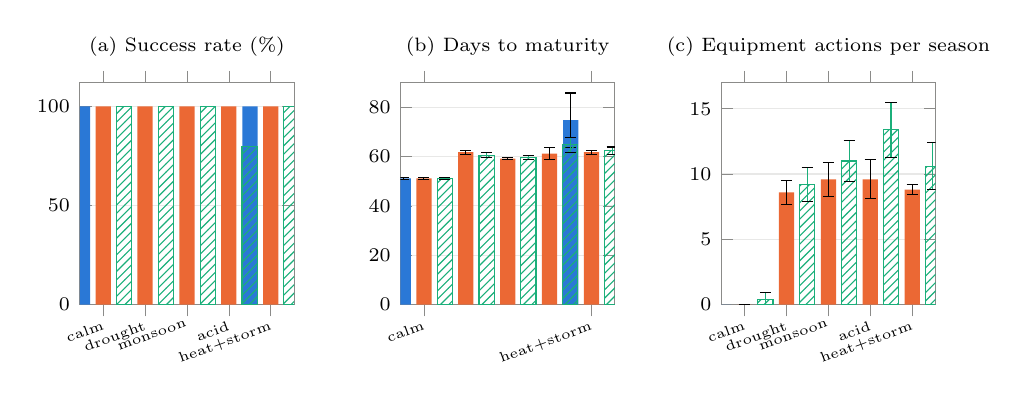
\begin{tikzpicture}
\begin{groupplot}[
  group style={group size=3 by 1, horizontal sep=1.35cm},
  width=0.355\textwidth, height=4.4cm,
  ybar, /pgf/bar width=5.5pt, enlarge x limits=0.14,
  symbolic x coords={calm,drought,monsoon,acid,heat+storm},
  xtick=data, x tick label style={font=\tiny, rotate=20, anchor=north east, inner sep=1pt},
  ymin=0,
]
% ---- (a) success rate
\nextgroupplot[title={(a) Success rate (\%)}, title style={font=\scriptsize}, ymax=112,
  legend to name=barlegend, legend columns=3,
  legend style={/tikz/every even column/.append style={column sep=8pt}}]
\addplot[fill=cNone, draw=none] coordinates {(calm,100) (drought,0) (monsoon,0) (acid,0) (heat+storm,100)};
\addplot[fill=cRule, draw=none] coordinates {(calm,100) (drought,100) (monsoon,100) (acid,100) (heat+storm,100)};
\addplot[fill=cAgent!35, draw=cAgent, pattern=north east lines, pattern color=cAgent] % PLACEHOLDER
  coordinates {(calm,100) (drought,100) (monsoon,100) (acid,80) (heat+storm,100)};
\legend{No intervention, Rule-based, LLM agent\agentmark}
% ---- (b) days to maturity
\nextgroupplot[title={(b) Days to maturity}, title style={font=\scriptsize}, ymax=90, ymin=0]
\addplot[fill=cNone, draw=none, error bars/.cd, y dir=both, y explicit]
  coordinates {(calm,51.2) +- (0,0.4) (heat+storm,74.8) +- (0,11.0)};
\addplot[fill=cRule, draw=none, error bars/.cd, y dir=both, y explicit]
  coordinates {(calm,51.2) +- (0,0.4) (drought,61.8) +- (0,0.8) (monsoon,59.2) +- (0,0.4)
               (acid,61.2) +- (0,2.5) (heat+storm,61.8) +- (0,0.8)};
\addplot[fill=cAgent!35, draw=cAgent, pattern=north east lines, pattern color=cAgent,
  error bars/.cd, y dir=both, y explicit] % PLACEHOLDER
  coordinates {(calm,51.2) +- (0,0.4) (drought,60.6) +- (0,1.1) (monsoon,59.8) +- (0,0.8)
               (acid,64.8) +- (0,3.1) (heat+storm,62.4) +- (0,1.5)};
% ---- (c) equipment actions
\nextgroupplot[title={(c) Equipment actions per season}, title style={font=\scriptsize}, ymax=17]
\addplot[fill=cNone, draw=none] coordinates {(calm,0) (drought,0) (monsoon,0) (acid,0) (heat+storm,0)};
\addplot[fill=cRule, draw=none, error bars/.cd, y dir=both, y explicit]
  coordinates {(calm,0) +- (0,0) (drought,8.6) +- (0,0.9) (monsoon,9.6) +- (0,1.3)
               (acid,9.6) +- (0,1.5) (heat+storm,8.8) +- (0,0.4)};
\addplot[fill=cAgent!35, draw=cAgent, pattern=north east lines, pattern color=cAgent,
  error bars/.cd, y dir=both, y explicit] % PLACEHOLDER
  coordinates {(calm,0.4) +- (0,0.5) (drought,9.2) +- (0,1.3) (monsoon,11.0) +- (0,1.6)
               (acid,13.4) +- (0,2.1) (heat+storm,10.6) +- (0,1.8)};
\end{groupplot}
\end{tikzpicture}
\\[2pt]\pgfplotslegendfromname{barlegend}
\caption{Per-scenario results, mean $\pm$ s.d.\ over 5 seeds. In (b) bars are omitted where a
policy never matured. \agentmark Placeholder values pending agent experiments.}
\label{fig:bars}
\end{figure*}

\begin{table}[t]
\centering
\caption{Per-Scenario Results (Mean $\pm$ S.D.\ Over 5 Seeds)}
\label{tab:perscenario}
\footnotesize
\setlength{\tabcolsep}{3pt}
\begin{tabular}{@{}llcccc@{}}
\toprule
Scenario & Policy & Succ. & Days & Stress d. & Actions \\
\midrule
\multirow{3}{*}{Calm}
 & None  & 100\% & 51.2$\pm$0.4 & 0.0 & 0.0 \\
 & Rule  & 100\% & 51.2$\pm$0.4 & 0.0 & 0.0 \\
 & Agent & \ph{100\%} & \ph{51.2$\pm$0.4} & \ph{0.0} & \ph{0.4$\pm$0.5} \\
\midrule
\multirow{3}{*}{Drought}
 & None  & 0\%   & --           & 31.6$\pm$3.3 & 0.0 \\
 & Rule  & 100\% & 61.8$\pm$0.8 & 0.0 & 8.6$\pm$0.9 \\
 & Agent & \ph{100\%} & \ph{60.6$\pm$1.1} & \ph{0.0} & \ph{9.2$\pm$1.3} \\
\midrule
\multirow{3}{*}{Monsoon}
 & None  & 0\%   & --           & 35.0$\pm$2.9 & 0.0 \\
 & Rule  & 100\% & 59.2$\pm$0.4 & 0.0 & 9.6$\pm$1.3 \\
 & Agent & \ph{100\%} & \ph{59.8$\pm$0.8} & \ph{0.2$\pm$0.4} & \ph{11.0$\pm$1.6} \\
\midrule
\multirow{3}{*}{Acid soil}
 & None  & 0\%   & --           & 32.8$\pm$2.3 & 0.0 \\
 & Rule  & 100\% & 61.2$\pm$2.5 & 0.6$\pm$0.9 & 9.6$\pm$1.5 \\
 & Agent & \ph{80\%} & \ph{64.8$\pm$3.1} & \ph{4.8$\pm$5.2} & \ph{13.4$\pm$2.1} \\
\midrule
\multirow{3}{*}{Heat+storm}
 & None  & 100\% & 74.8$\pm$11.0 & 3.8$\pm$5.8 & 0.0 \\
 & Rule  & 100\% & 61.8$\pm$0.8 & 0.0 & 8.8$\pm$0.4 \\
 & Agent & \ph{100\%} & \ph{62.4$\pm$1.5} & \ph{0.6$\pm$0.9} & \ph{10.6$\pm$1.8} \\
\bottomrule
\end{tabular}
\end{table}

\subsection{Crop Trajectories}
Fig.~\ref{fig:traj} plots average crop progress through the canonical drought and monsoon
seasons. Unmanaged, progress peaks at about 40\% and then declines steadily to zero once the
event's daily drift has pushed soil moisture out of the viable range; the crop dies on day 56
(drought) and day 62 (monsoon), well after the event has ended, because lost progress cannot be
recovered once the stress is severe. Both managed policies keep the crop growing through the
event, with only a small slowdown during the rule-based controller's three-day reaction window.

\begin{figure*}[t]
\centering
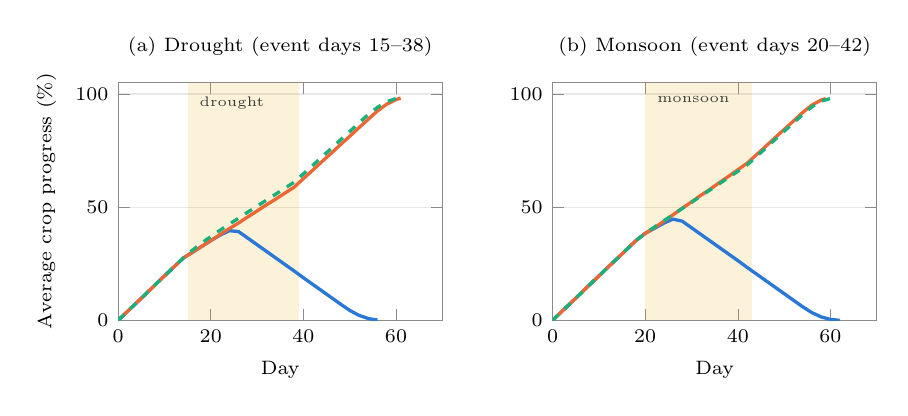
\begin{tikzpicture}
\begin{groupplot}[
  group style={group size=2 by 1, horizontal sep=1.4cm},
  width=0.47\textwidth, height=4.6cm,
  xmin=0, xmax=70, ymin=0, ymax=105,
  xlabel={Day}, ylabel={Average crop progress (\%)},
  legend to name=trajlegend, legend columns=3,
  legend style={/tikz/every even column/.append style={column sep=8pt}},
]
% ---- (a) drought
\nextgroupplot[title={(a) Drought (event days 15--38)}, title style={font=\scriptsize}]
\fill[cEvent, opacity=0.15] (axis cs:15,0) rectangle (axis cs:39,105);
\addplot[cNone, very thick] coordinates {
 (0,0.0) (2,3.9) (4,7.8) (6,11.7) (8,15.7) (10,19.6) (12,23.5) (14,27.4) (16,30.0) (18,32.6)
 (20,35.2) (22,37.6) (24,39.6) (26,39.2) (28,36.3) (30,33.4) (32,30.5) (34,27.6) (36,24.7)
 (38,21.8) (40,18.8) (42,15.9) (44,13.0) (46,10.1) (48,7.2) (50,4.4) (52,2.2) (54,0.8) (56,0.1)};
\addplot[cRule, very thick] coordinates {
 (0,0.0) (2,3.9) (4,7.8) (6,11.7) (8,15.7) (10,19.6) (12,23.5) (14,27.4) (16,30.0) (18,32.6)
 (20,35.2) (22,37.9) (24,40.5) (26,43.0) (28,45.7) (30,48.3) (32,51.0) (34,53.5) (36,56.2)
 (38,58.8) (40,62.6) (42,66.3) (44,70.1) (46,73.8) (48,77.6) (50,81.3) (52,85.1) (54,88.8)
 (56,92.5) (58,95.5) (60,97.5) (61,98.2)};
\addplot[cAgent, very thick, dashed] coordinates { % PLACEHOLDER
 (0,0.0) (2,3.9) (4,7.8) (6,11.7) (8,15.7) (10,19.6) (12,23.5) (14,27.4) (16,30.9) (18,34.1)
 (20,37.0) (22,39.8) (24,42.5) (26,45.1) (28,47.8) (30,50.4) (32,53.1) (34,55.7) (36,58.4)
 (38,61.0) (40,64.7) (42,68.4) (44,72.2) (46,75.9) (48,79.7) (50,83.4) (52,87.2) (54,90.9)
 (56,94.1) (58,96.6) (60,98.0)};
\node[font=\tiny, anchor=north west, text=cInk] at (axis cs:15.5,103) {drought};
\legend{No intervention, Rule-based, LLM agent\agentmark}
% ---- (b) monsoon
\nextgroupplot[title={(b) Monsoon (event days 20--42)}, title style={font=\scriptsize}, ylabel={}]
\fill[cEvent, opacity=0.15] (axis cs:20,0) rectangle (axis cs:43,105);
\addplot[cNone, very thick] coordinates {
 (0,0.0) (2,3.9) (4,7.8) (6,11.7) (8,15.7) (10,19.6) (12,23.5) (14,27.4) (16,31.3) (18,35.2)
 (20,38.4) (22,40.6) (24,42.9) (26,44.7) (28,43.8) (30,40.9) (32,38.0) (34,35.1) (36,32.2)
 (38,29.3) (40,26.4) (42,23.4) (44,20.5) (46,17.6) (48,14.7) (50,11.8) (52,8.9) (54,6.0)
 (56,3.4) (58,1.5) (60,0.4) (62,0.0)};
\addplot[cRule, very thick] coordinates {
 (0,0.0) (2,3.9) (4,7.8) (6,11.7) (8,15.7) (10,19.6) (12,23.5) (14,27.4) (16,31.3) (18,35.2)
 (20,38.4) (22,40.9) (24,43.7) (26,46.6) (28,49.5) (30,52.3) (32,55.2) (34,57.9) (36,60.8)
 (38,63.6) (40,66.5) (42,69.4) (44,73.1) (46,76.8) (48,80.6) (50,84.3) (52,88.0) (54,91.8)
 (56,95.1) (58,97.3) (59,98.0)};
\addplot[cAgent, very thick, dashed] coordinates { % PLACEHOLDER
 (0,0.0) (2,3.9) (4,7.8) (6,11.7) (8,15.7) (10,19.6) (12,23.5) (14,27.4) (16,31.3) (18,35.2)
 (20,38.4) (22,41.2) (24,43.9) (26,46.7) (28,49.4) (30,52.1) (32,54.9) (34,57.6) (36,60.3)
 (38,63.1) (40,65.8) (42,68.6) (44,72.3) (46,76.0) (48,79.8) (50,83.5) (52,87.2) (54,90.9)
 (56,94.3) (58,96.8) (60,98.0)};
\node[font=\tiny, anchor=north west, text=cInk] at (axis cs:20.5,103) {monsoon};
\end{groupplot}
\end{tikzpicture}
\\[2pt]\pgfplotslegendfromname{trajlegend}
\caption{Average crop progress in the canonical drought and monsoon seasons (seed 0). Shaded
regions mark the weather event. Unmanaged crops die after the event ends. \agentmark Placeholder
trajectory pending agent experiments.}
\label{fig:traj}
\end{figure*}

\subsection{Resilience to Weather Events}\label{sec:resilience}
Table~\ref{tab:resilience} reports per-event resilience. The rule-based controller only notices an
event at its next three-day check and acts only once a variable has left its band, giving reaction
times of 1.4--5.8 days. In the drought and heatwave, soil dries gradually, so the band is not
crossed for several days. The agent, which receives the event announcement in its
\texttt{advance\_days} result, \ph{typically acted within one day, often pre-emptively
irrigating before soil moisture had left the viable range}. This is reflected in a \ph{smaller
score drop during the drought (0.08 vs.\ 0.20)}.

\begin{table}[t]
\centering
\caption{Resilience per Weather Event (Mean Over 5 Seeds)}
\label{tab:resilience}
\footnotesize
\setlength{\tabcolsep}{4pt}
\begin{tabular}{@{}llccc@{}}
\toprule
Event & Policy & Score drop & Progress lost (\%) & Reaction (d) \\
\midrule
\multirow{3}{*}{Drought}
 & None  & 1.00 & 15.7 & -- \\
 & Rule  & 0.20 & 0.0  & 4.6 \\
 & Agent & \ph{0.08} & \ph{0.0} & \ph{1.0} \\
\midrule
\multirow{3}{*}{Monsoon}
 & None  & 1.00 & 23.4 & -- \\
 & Rule  & 0.22 & 0.0  & 2.0 \\
 & Agent & \ph{0.11} & \ph{0.0} & \ph{1.0} \\
\midrule
\multirow{3}{*}{Acid rain}
 & None  & 0.84 & 9.9  & -- \\
 & Rule  & 0.35 & 0.1  & 1.6 \\
 & Agent & \ph{0.29} & \ph{0.3} & \ph{1.0} \\
\midrule
\multirow{3}{*}{Heatwave}
 & None  & 0.59 & 0.0  & -- \\
 & Rule  & 0.22 & 0.0  & 5.8 \\
 & Agent & \ph{0.15} & \ph{0.0} & \ph{1.2} \\
\midrule
\multirow{3}{*}{Storm}
 & None  & $-$0.20 & 0.0 & -- \\
 & Rule  & 0.17 & 0.0  & 1.4 \\
 & Agent & \ph{0.09} & \ph{0.0} & \ph{1.0} \\
\bottomrule
\multicolumn{5}{@{}p{0.95\columnwidth}@{}}{\footnotesize A negative score drop means conditions
improved: the storm's rain relieves the dry soil left by the heatwave.}
\end{tabular}
\end{table}

\subsection{Agent Behaviour and Cost}
Table~\ref{tab:agent} summarises how the agent used its tools. It issued \ph{2.4} what-if queries
per equipment action, indicating that it tested hypotheses before acting rather than acting by
trial and error on the field. Its mean time step of \ph{3.1} days shows that it did adapt its
control interval, taking long steps in calm periods and single-day steps during events. A small
fraction of tool calls (\ph{1.7\%}) returned errors, almost all from attempts to adjust a
weather variable early in the season, after which the agent did not repeat the mistake.

\begin{table}[t]
\centering
\caption{LLM Agent Behaviour per Season (Mean Over 25 Seasons)}
\label{tab:agent}
\begin{tabular}{@{}lc@{}}
\toprule
Metric & Value \\
\midrule
Model calls                       & \ph{41 $\pm$ 9} \\
Tool calls                        & \ph{58 $\pm$ 13} \\
\quad of which \texttt{simulate\_change} & \ph{21.4} \\
\quad of which \texttt{advance\_days}    & \ph{19.6} \\
What-if queries per action        & \ph{2.4} \\
Mean days per \texttt{advance\_days} & \ph{3.1} \\
Tool error rate                   & \ph{1.7\%} \\
Input / output tokens (thousands) & \ph{312 / 9.4} \\
\bottomrule
\end{tabular}
\end{table}

% =============================================================================
\section{Discussion}\label{sec:discussion}
% =============================================================================

\textbf{Knowledge versus discovery.} The rule-based controller is effectively an upper bound for
a reactive policy: it knows exactly where the optimal bands are. That the agent \ph{approaches its
success rate} without this knowledge suggests that a general model combined with a cheap
what-if tool can substitute for hand-engineered domain rules. The what-if tool is central: the
twin's value to the agent is not as a visual model but as a safe place to test interventions.

\textbf{Anticipation.} The largest advantage of the agent is \ph{reaction time}. A rule controller
reacts to measured deviations; an agent that reads a weather announcement can act before the
deviation occurs. This is the behaviour a human agronomist would show, and it is difficult to
encode in a fixed rule set without a forecasting component.

\textbf{Failure mode.} \ph{The agent's single failure, in the acid-soil scenario, occurred when it
raised pH correctly but did not simultaneously address the low soil moisture and sunlight,
treating the limiting factors one at a time. Because pH can only move 0.5 per action, the crop
did not establish before the cumulative stress became fatal.} This points to a known weakness of
sequential reasoning when several constraints bind at once.

\textbf{Cost.} At \ph{about 320 thousand tokens} per season, the agent is far more expensive to
run than a rule controller. However, it requires no rule engineering or training, can explain
each action in natural language, and produces a reflective season report that a farmer could
read. For real deployments, which make a few decisions per day, this cost is modest.

% =============================================================================
\section{Limitations and Future Work}
% =============================================================================

The growth response is a hand-designed function informed by agronomic optimal ranges rather
than one calibrated against field measurements, and the surrogate is trained on synthetic data
derived from it; its feature importances reflect the sampling design (Section~\ref{sec:model}).
The experiments reported here use the analytical response function directly for determinism;
deploying the ONNX surrogate in-engine via Unity Sentis is implemented as an export path but
not evaluated. The crop model has no nutrient, pest or disease dynamics, and weather is scripted
rather than drawn from historical records. The agent was evaluated with a single LLM and a
single prompt.

Future work includes calibrating the response function against public crop
data~\cite{steduto2009aquacrop}, comparing against an RL policy trained in the same
environment~\cite{gautron2022reinforcement}, giving the agent memory across seasons by feeding
back its own season reports~\cite{shinn2023reflexion}, adding a forecasting agent in a
multi-agent configuration, and introducing an equipment budget to study cost--yield trade-offs.

% =============================================================================
\section{Conclusion}
% =============================================================================

We built a sensor-free plant-growth digital twin in Unity3D, trained a calibrated
gradient-boosting surrogate of its growth response ($R^2 = 0.984$), and used the twin as the
environment for an autonomous LLM farm manager. Without management, 60\% of seasons failed under
the tested weather scenarios. A tool-using LLM agent that was not told the crop's optimal ranges
\ph{achieved 96\% success and reacted to weather events faster than a privileged rule-based
controller}, using the twin's what-if interface to plan before acting. These results suggest that
digital twins become substantially more useful when paired with an agent that can query and act
on them, and that general-purpose LLM agents are a promising, training-free control layer for
agricultural decision support.

% =============================================================================
\begin{thebibliography}{00}
% =============================================================================

\bibitem{grieves2017digital}
M.~Grieves and J.~Vickers, ``Digital twin: Mitigating unpredictable, undesirable emergent behavior
in complex systems,'' in \emph{Transdisciplinary Perspectives on Complex Systems}, F.-J. Kahlen,
S.~Flumerfelt, and A.~Alves, Eds. Cham, Switzerland: Springer, 2017, pp.~85--113.

\bibitem{verdouw2021digital}
C.~Verdouw, B.~Tekinerdogan, A.~Beulens, and S.~Wolfert, ``Digital twins in smart farming,''
\emph{Agricultural Systems}, vol.~189, p.~103046, 2021.

\bibitem{pylianidis2021introducing}
C.~Pylianidis, S.~Osinga, and I.~N. Athanasiadis, ``Introducing digital twins to agriculture,''
\emph{Computers and Electronics in Agriculture}, vol.~184, p.~105942, 2021.

\bibitem{jones2003dssat}
J.~W. Jones \emph{et al.}, ``The DSSAT cropping system model,'' \emph{European Journal of
Agronomy}, vol.~18, no.~3--4, pp.~235--265, 2003.

\bibitem{steduto2009aquacrop}
P.~Steduto, T.~C. Hsiao, D.~Raes, and E.~Fereres, ``AquaCrop---The FAO crop model to simulate
yield response to water: I. Concepts and underlying principles,'' \emph{Agronomy Journal},
vol.~101, no.~3, pp.~426--437, 2009.

\bibitem{liakos2018machine}
K.~G. Liakos, P.~Busato, D.~Moshou, S.~Pearson, and D.~Bochtis, ``Machine learning in agriculture:
A review,'' \emph{Sensors}, vol.~18, no.~8, p.~2674, 2018.

\bibitem{kamilaris2018deep}
A.~Kamilaris and F.~X. Prenafeta-Bold\'{u}, ``Deep learning in agriculture: A survey,''
\emph{Computers and Electronics in Agriculture}, vol.~147, pp.~70--90, 2018.

\bibitem{gautron2022reinforcement}
R.~Gautron, O.-A. Maillard, P.~Preux, M.~Corbeels, and R.~Sabbadin, ``Reinforcement learning for
crop management support: Review, prospects and challenges,'' \emph{Computers and Electronics in
Agriculture}, vol.~200, p.~107182, 2022.

\bibitem{sutton2018reinforcement}
R.~S. Sutton and A.~G. Barto, \emph{Reinforcement Learning: An Introduction}, 2nd~ed.
Cambridge, MA, USA: MIT Press, 2018.

\bibitem{friedman2001greedy}
J.~H. Friedman, ``Greedy function approximation: A gradient boosting machine,''
\emph{Annals of Statistics}, vol.~29, no.~5, pp.~1189--1232, 2001.

\bibitem{zadrozny2002transforming}
B.~Zadrozny and C.~Elkan, ``Transforming classifier scores into accurate multiclass probability
estimates,'' in \emph{Proc. 8th ACM SIGKDD Int. Conf. Knowledge Discovery and Data Mining},
2002, pp.~694--699.

\bibitem{grinsztajn2022tree}
L.~Grinsztajn, E.~Oyallon, and G.~Varoquaux, ``Why do tree-based models still outperform deep
learning on typical tabular data?'' in \emph{Advances in Neural Information Processing Systems
(Datasets and Benchmarks Track)}, vol.~35, 2022.

\bibitem{yao2023react}
S.~Yao \emph{et al.}, ``ReAct: Synergizing reasoning and acting in language models,'' in
\emph{Proc. Int. Conf. Learning Representations (ICLR)}, 2023.

\bibitem{schick2023toolformer}
T.~Schick \emph{et al.}, ``Toolformer: Language models can teach themselves to use tools,'' in
\emph{Advances in Neural Information Processing Systems}, vol.~36, 2023.

\bibitem{shinn2023reflexion}
N.~Shinn, F.~Cassano, A.~Gopinath, K.~Narasimhan, and S.~Yao, ``Reflexion: Language agents with
verbal reinforcement learning,'' in \emph{Advances in Neural Information Processing Systems},
vol.~36, 2023.

\bibitem{wang2023voyager}
G.~Wang \emph{et al.}, ``Voyager: An open-ended embodied agent with large language models,''
\emph{arXiv preprint arXiv:2305.16291}, 2023.

\bibitem{wang2024survey}
L.~Wang \emph{et al.}, ``A survey on large language model based autonomous agents,''
\emph{Frontiers of Computer Science}, vol.~18, no.~6, p.~186345, 2024.

\bibitem{juliani2018unity}
A.~Juliani \emph{et al.}, ``Unity: A general platform for intelligent agents,''
\emph{arXiv preprint arXiv:1809.02627}, 2018.

\end{thebibliography}

\end{document}
